\chapter{Refactoring Library} \label{chapter:refactoring-library}

The refactoring library is the heart of the Scala Refactoring project. It contains the means to analyze a Scala program, to transform it and to turn these modifications back into source code. When writing a refactoring, one usually has to take care of the following steps:

\begin{itemize}
 \item provide a user interface so that a specific refactoring can be discovered and invoked from the IDE.
 \item analyze the program under refactoring to find out whether the refactoring is applicable and further to determine the parameters and constraints for the refactoring.
 \item transform the program tree from its original form into a new -- refactored -- form according to the refactoring's configuration.
 \item turn this new form back into source code, keeping as much of the original formatting in place as possible and to generate code for new parts of the program.
 \item present the result of the refactoring to the user -- typically in the form of a patch --  and apply it to the source code.
\end{itemize}

From all these steps, the first and the last one are IDE-platform dependent and usually well supported (see Chapter XXX). For the remaining three, the refactoring library contains the necessary infrastructure to make these steps as simple as possible.

The essence of a refactoring is a transformation that takes a program in some abstract form and changes its structure. To know what to transform, one has to analyze the program first. That we also have to turn a refactored program back into source code is a consequence of storing programs as plain text files, but not an essential part of a refactoring. Therefore, one of the design goals was to provide a generic implementation that can handle all kinds of changes without knowing exactly what the transformation changed.

In the remainder of this chapter, we shall first take a look at the architecture of the library and then describe each of the three main components in detail.

\section{Overview}

% Muss ich den AST erkl�ren? Warum es den braucht und so?

Automated refactoring implementations typically do not work on the source code directly but -- just as a compiler -- do the majority of the work on the abstract syntax tree (AST) of the program. We also do not create our own AST representation but reuse the Scala compiler's parser and type checker (as explained in Chapter XXX, we also do not parse the code ourselves but get the AST from the IDE). This not only saved time during the development, but also makes it easier to implement a new refactoring if one is already familiar with the Scala compiler's AST.

The Scala AST is heterogeneous, meaning that ...

 The Scala compiler provides some infrastructure to traverse and transform the AST.

Scala's AST is explained in more detail in Appendix~\vref{chapter:scala-ast}, but a general knowledge of what an AST is should suffice to follow the explanations in this chapter. Useful to know is that all trees have a position information: either indicating a location from where the tree origins or a \src{NoPosition}, which denotes trees that do not have a corresponding source code location. This information is later used by the transformation and code generation phases.%: trees with a \src{NoPosition} are pretty printed and the trees with a specific source location are reused (this is needed to preserve the formatting of the source code).

As we have seen at the beginning of this chapter, a typical refactoring takes the current file's AST and the user's selection or caret position and first checks if the chosen refactoring is applicable -- e.g. whether the selected region of the source file corresponds to an AST element that can be handled by the chosen refactoring. If necessary, the refactoring queries aditional configuration from the user -- e.g. extracting a methind needs a new name. The AST is then transformed into its new form and handed over to the source generator to turn the AST back into source code (see \figref{figure:refactoring-flow} for a visualization of this workflow). As motivated above, generating the source code is already implemented generically and needs no further instructions from the refactoring implementer. %zu viel wiederholund von oben?

\begin{figure}
  \centering
  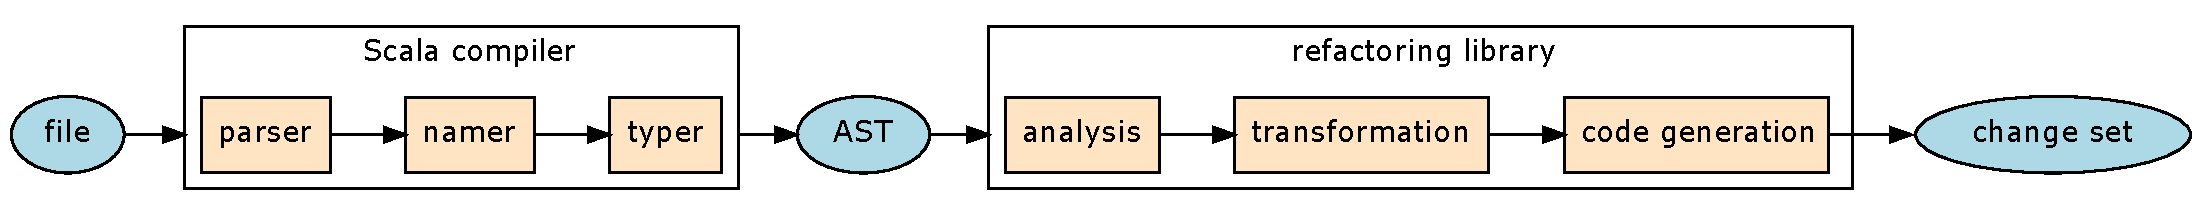
\includegraphics[width=\linewidth]{refactoring-flow.pdf}
  \caption{The work-flow of the refactoring. The IDE uses the compiler to parse the source file and passes the resulting syntax tree to the refactoring tool. The result of a refactoring is a set of changes, viz. a patch, that the IDE has to apply to the source files (adapted from \cite{ScalaRefactoring}).}
  \label{figure:refactoring-flow}
\end{figure}

The architecture (see \figref{figure:refactoring-architecture}) and also the source code layout follow these three phases of the refactoring:

\begin{description}
 \item[Analysis] in package \src{analysis} contains the means to analyze the program and to build an index for the identifiers in the program. This will be explained further in Section \vref{section:analysis}.
 \item[Transformation] in package \src{transformation} provides a framework to write, combine and apply transformations on trees, as well as some factory methods to create new trees. How these work is described in Section \vref{section:transformation}.
 \item[Source Generation] in package \src{sourcegen} mainly contains the \src{SourceGenerator} that turns an AST back into change objects (i.e. patches) for the source code as explained in Section \vref{section:source-generation}.
\end{description}

\begin{figure}
  \centering
  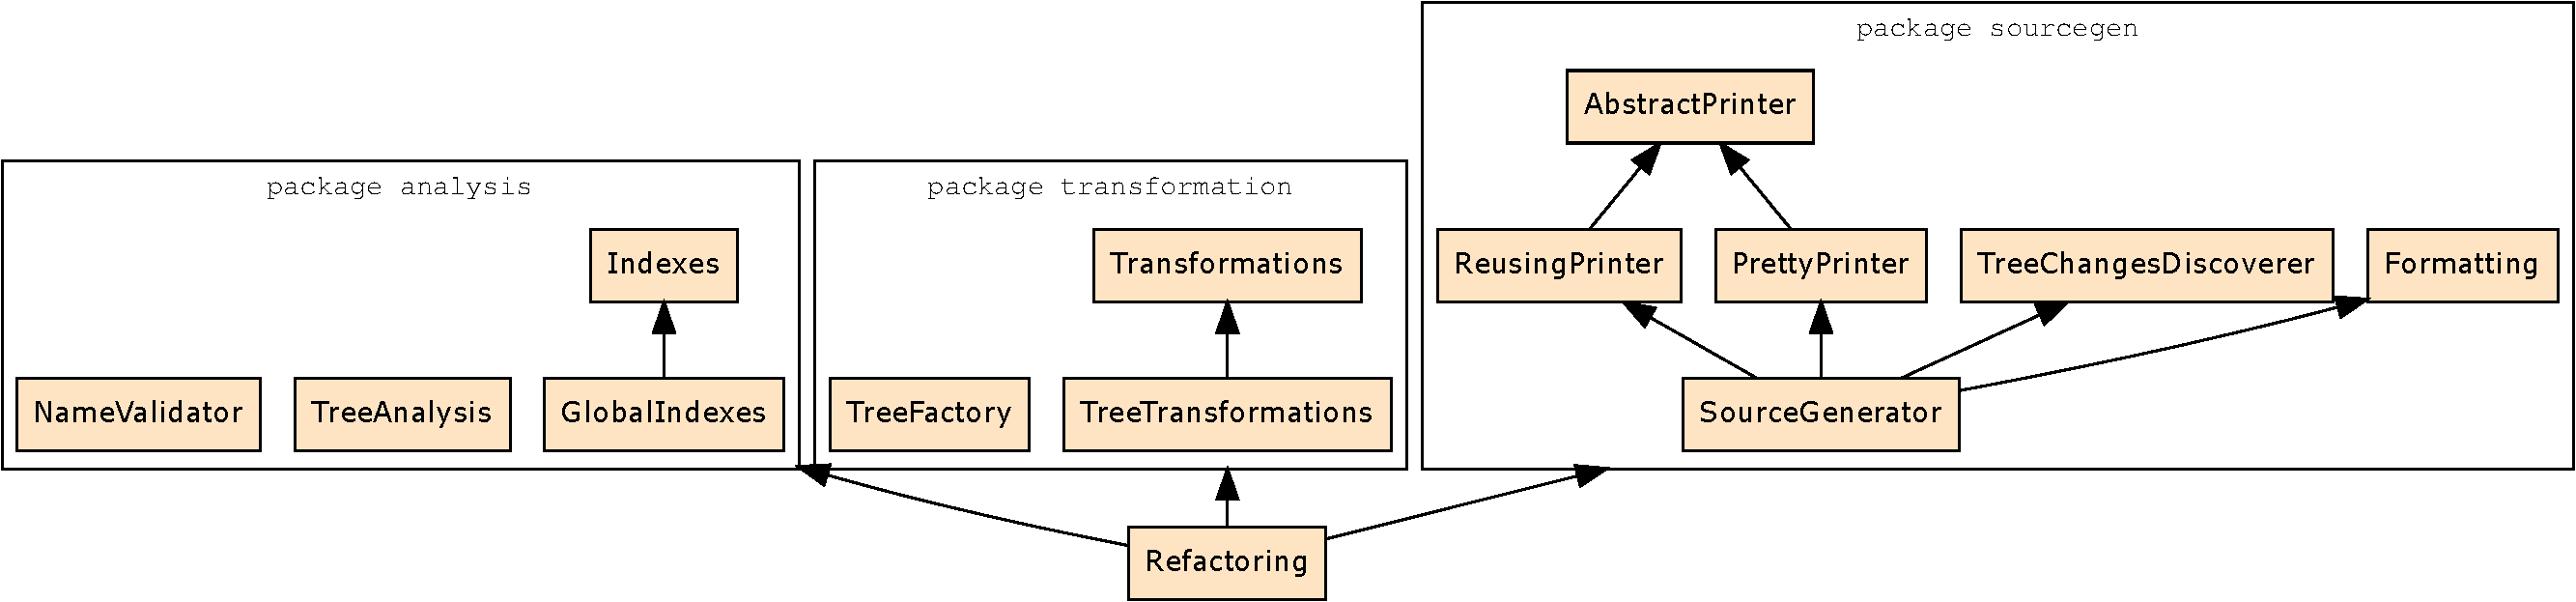
\includegraphics[width=\linewidth]{refactoring-architecture.pdf}
  \caption{An overview of the refactoring library architecture: the three main packages \src{analysis}, \src{transformation}, and \src{sourcegen}. Note that there exist more traits and classes in these packages -- but for the sake of clarity, only the major ones are shown.}
  \label{figure:refactoring-architecture}
\end{figure}

% path dependent type, global?

In the remainder of this chapter, the three library components will be explained in more detail. %Keep in mind that the shown functionality is not meant to be feature complete but can and will be extended as seen fit. %geh�rt das hier hin?

\section{Analysis} \label{section:analysis}

An import step in each refactoring is to analyze the current program that is being refactored. For example, when doing a Rename refactoring, we need to resolve all references to the renamed name. A more complex example is Extract Method, where we need to perform data-flow analysis to determine the parameters and return values of the extracted method.

Our IDEs also analyze the program code in a similar way to make the life of the programmer easier: finding the declaration of a variable or listing all subtypes of a class are common operations.

Our analyses heavily depend on the Scala compiler's AST and all the information it provides through the program's symbols. For example, each symbol has an owner that can be used to navigate the logical structure of the program. There are also almost one hundred \src{isXY} methods defined on the \src{Symbol} class that can be used to query information:

\begin{lstlisting}
abstract class Symbol {
  %\ldots%
  def isAnonymousClass: Boolean
  def isConstructor: Boolean
  def isGetter: Boolean
  def isLocal: Boolean
  def isSubClass(that: Symbol): Boolean
  %\ldots%
}
\end{lstlisting}

All the trees that inherit from the \src{SymTree} trait provide a symbol instance, where \src{DefTrees} usually introduce a new symbol and \src{RefTrees} reference a symbol from a \src{DefTree}. The following illustration shows how symbols are related (not all symbols are colored, for example, the built in types have a symbol as well):

\begin{lstlisting}
trait %\bluebox{SuperClass}% {
  def %\greenbox{strlen}%(%\redbox{str}%: String) = %\redbox{str}%.length
  def %\lgreenbox{abstractMethod}%: Int
}

class %\yellowbox{SubClass}% extends %\bluebox{SuperClass}% {
  def %\greybox{abstractMethod}% = 1 + %\greenbox{strlen}%("1")
}
\end{lstlisting}

Note that the two \src{abstractMethod} symbols are not the same, but there are other means to find overriden and implemented methods in subclasses, as we shall see later.

While the trees can have a reference to a symbol, the converse is not true: symbols do not know about the trees they are related to. But for refactoring, this information is crucial. This is why the refactoring library contains the means to build an index that relates symbols and corresponding trees.

\subsection{Refactoring Index Interface}

Building an index over a whole project can be expensive, so ideally, the IDE would maintain the index and pass it to the refactoring library when need, in the same way that the library does not compile the source files itself but gets the ASTs directly from the IDE.

The interface that needs to be implemented and is used by the refactorings to query the index looks as follows (note that \src{global} is an instance of the compiler that is provided by an outer trait so the trees can be used as path dependent types (see Appendix \vref{section:path-dependent-types})):

\begin{lstlisting}
trait IndexLookup {
  /**
    * Returns all defined symbols, i.e. symbols of DefTrees.
    * */
  def allDefinedSymbols(): List[global.Symbol]
  
  /**
    * Returns all symbols that are part of the index, either referenced or defined.
    * */
  def allSymbols(): List[global.Symbol]    
  
  /**
    * For a given Symbol, tries to find the tree that declares it.
    * */
  def declaration(s: global.Symbol): Option[global.DefTree]
  /**
    * For a given Symbol, returns all trees that contain a reference to it.
    * */
  def references(s: global.Symbol): List[global.Tree]
  
  /**
    * For a given Symbol, returns all trees that reference or declare the Symbol.
    * */
  def occurences(s: global.Symbol): List[global.Tree]

  /**
    * For the given Symbol - which can be a class or object - returns a list of all sub- 
    * and super classes, in no particular order.
    */
  def completeClassHierarchy(s: global.Symbol): List[global.Symbol] =
    (s :: (allDefinedSymbols filter (_.ancestors contains s) flatMap (s => s :: s.ancestors)) 
      filter (_.pos != global.NoPosition) distinct)

}
\end{lstlisting}

The library also contains a default implementation that can be used if the IDE does not already maintain an index itself, as described in the following section.

\subsection{Default Index Implementation}

Building an index can be expensive: whenever a compilation unit in the program changes, references to the symbols from other compilation units can change, and also the other way around. Because of this, it is expensive to maintain one monolithic index that needs to be recreated on every change in the program. The provided implementation avoids this by maintaining a data structure for each compilation unit and combining these for queries. The implementation comprises these parts:

\begin{description}
 \item[CompilationUnitIndex] One index per compilation unit that holds the references and declarations of just this part of the program.. This structure can be rebuilt everytime a compilation unit changes. Rebuilding it traverses the whole tree once and stores mappings from symbols to \src{RefTrees} and \src{DefTrees}.
 \item[GlobalIndex] An implementation of the \src{IndexLokup} trait that ties together any number of these per compilation unit indices, but is completely stateless itself.
\end{description}

Whenever a compilation unit changes, just a single \src{CompilationUnitIndex} needs to be rebuilt and combined with the already existing ones into a new \src{GlobalIndex}.

\subsection{Resolving References}

Resolving the declaration tree of a symbol is an inexpensive lookup, but the reverse -- finding all references -- causes more work. In \src{GlobalIndex}, the process of finding all references is done in multiple steps: first, the symbol is \textit{expanded} and second all references to these expanded symbols are collected. What do we mean by expanding a symbol? Consider the example of the colored symbols we mentioned at the beginning of Section \ref{section:analysis}. The implementing method defines a different symbol than the abstract declared method. But when we want to find references, we need all references to both symbols. The same is true for getters and setters: renaming a class parameter also needs to rename all usages of getters and setters. To do this, the index implementation uses so called \src{SymbolExpanders}:

\begin{lstlisting}
trait SymbolExpander {
  def expand(s: Symbol): List[Symbol] = List(s)
}
\end{lstlisting}

The \src{SymbolExpander} is used as a stackable trait (see Appendix \vref{section:stackable-traits}) and is at the time of this writing implemented in the following variations:

\begin{description}
 \item[ExpandGetterSetters] connects getters, setters and the underlying field as well as constructor parameters. This can be done with the symbol alone and 
 \item[SuperConstructorParameters] resolves class parameters that are passed to a superconstructor.
 \item[Companion] to find the companion objects or class for a symbol.
 \item[OverridesInClassHierarchy] searches for a symbol in all sub- and superclasses. that might override or implement it.
\end{description}

The \src{GlobalIndex} uses all these traits, but it would also be possible for an implementation of the index to use only a subset of these to improve the performance. So when for example all references to a method need to be found, the initial symbol is run through all the expanders until a fix point is reached.

The following graphic illustrates the process with an example; circles represent symbols and squares trees. We start with a single symbol on the left -- e.g. a class field -- and in the first step, it is expanded to two symbols -- for example because the class field has a getter method. We do another round of expansion and find yet another related symbol (the getter might be overridden in a subclass). The third expansion yields no new symbols, thus the fourth step concludes by collecting all references and declarations to these symbols.

\begin{center}
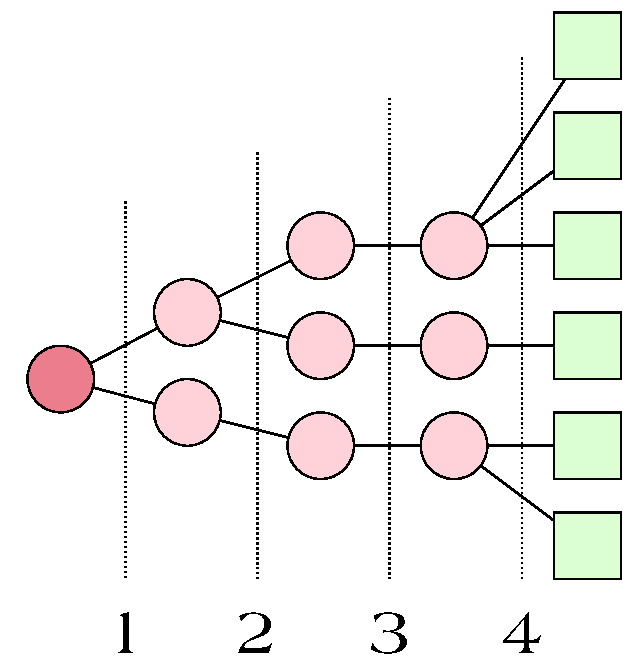
\includegraphics[width=0.5\linewidth]{expanding_symbols.pdf}
\end{center}

\subsection{Tree Analysis}

Besides the index to lookup references and declarations, some refactorings need more sophisticated analysis of the program. This section introduces the \src{TreeAnalysis} trait which contains these functionality.

\subsubsection{Local Dependencies}

The Extract Method refactoring extracts a selection of expressions into a new method. To do this, it needs to calculate all dependencies the selected expressions have to their enclosing scopes. Variables and functions that are not accessible from the new method location need to be passed as arguments, and program elements that are declared inside the extracted method and used outside of the selection need to be passed back.

In the following listing, the user wants to extract the selected expressions:

\begin{lstlisting}
def calculate {
  val sumList: Seq[Int] => Int = _ reduceLeft (_+_)
  val prodList: Seq[Int] => Int = _ reduceLeft (_*_)
  val values = 1 to 10 toList
  %\bluebox{val     sum = sumList(values)}%
  %\bluebox{val product = prodList(values)}%

  println("The sum from 1 to 10 is "+ sum +".")
}
\end{lstlisting}

The refactoring has to create a method that takes the \src{values} and the \src{sumList} and \src{prodList} functions as arguments. Also, because the \src{sum} value is used in the originating method -- but not \src{product} -- it has to be returned from the new method.

The calculation of these inbound and outbound dependencies is done as follows:

\paragraph{Inbound:} Find all symbols that are declared in the current scope (e.g. the method we extract from) and remove all declarations that are defined inside the selection. This gives us all the inbound parameters.

\paragraph{Outbound:} For each symbol that is definde inside the selection, check if it is used anywhere outside the selection.

\subsection{Name Validation}

When doing refactoring, one often has to introduce new names into the program, that can potentially conflict with an already existing name that is currently in scope. The \src{NameValidation} trait offers the functionality to check whether a name is a valid identifier -- based on the Scala compiler -- and checking if a name will collide with an already existing name:

\begin{lstlisting}

\end{lstlisting}



\section{Transformation} \label{section:transformation}

At the heart of every refactoring lies a \textit{transformation} that takes the current program in its abstract syntax tree form and transforms it into its refactored form. Such a transformation can be as simple as changing names -- think of the Rename refactoring -- or restructure large parts of the AST as in an Extract or Move refactoring. 

Often, a larger refactoring comprises many smaller transformations. An illustrative example is the Extract Method refactoring, which can be assembled from three basic transformations:

\begin{description}
 \item[Create Method] to introduce a new (empty) method.
 \item[Copy Statements] to copy the selected statements into the newly created method.
 \item[Replace Statements] to replace the original statements that have been copied to the new method with a call to it.
\end{description}

The \textit{replace} transformation itself is again a combination of two even more fundamental transformations: \textit{insert} and \textit{delete}. Once we have our Extract Method transformation, it can then again be combined with other transformations -- for example into an Extract Class refactoring. It should be clear from this that the key to a reusable refactoring library lies in the composability of its transformations. 

Conceptually, chaining simple transformations to build more powerful ones follows the Unix pipes philosophy. The design of this implementation was inspired by the Stratego program transformation tool-set (referenz) and the Kiama language processing library (referenz). Functional programming also uses the term \textit{combinator} to denote functions that can be combined and yield new functions of the same kind. An example of this are parser combinators (referenz), which are part of the Scala standard library.

In contrast to unix pipes that operate on their input line by line, performing transformations on a tree datastructure adds an additional dimension. When transforming trees, we are also concerned with questions on how we want to traverse the tree -- i.e. pre-order or post-order -- and to which children a transformation should be applied. The presented implementation handles all these concerns in a uniform way.

In the remainder of this section, we will develop the basics of the Scala refactoring's transformation combinators and show examples of their usage.

\subsection{Transformations}

A refactoring transformation is essentially a function that transforms a tree into an other tree. But because most transformations do not apply to all kinds of possible trees, we model a transformation as a function of type $Tree\Rightarrow Option[Tree]$, making use of Scala's \src{Option} monad to indicate the potential inability to transform. In the actual implementation, the transformations are implemented generically as a \src{Transformation[A,~B]} that extend \src{A~$\Rightarrow$~Option[B]}:

\begin{lstlisting}
abstract class Transformation[A, B] extends (A %$\Rightarrow$% Option[B]) {
  self %$\Rightarrow$%

  def apply(in: A): Option[B]
%\ldots%
}
\end{lstlisting}

The explicit self type annotation (see Appendix \vref{section:self-type-annotation}) will be used later in the implementation of the combinators. Note that all transformations are implemented polymorphic, but to make the explanations more clear, we will assume that they are used to transform trees.

Transformations can be created from partial functions using the \src{transformation} convenience function. As an example, we create a transformation that reverses the order of a class, trait, or object's member definitions and apply it to a given template instance.

\begin{lstlisting}
def transformation[A, B](f: PartialFunction[A, B]) = new Transformation[A, B] {
  def apply(t: A): Option[B] = f lift t
}

val reverseTemplateMembers = transformation[Tree, Tree] {
  case t: Template %$\Rightarrow$% t copy (body = t.body.reverse)
}

val result: Option[Tree] = reverseTemplateMembers(template)
\end{lstlisting}

Now that we have a way to create single transformations, we need to be able to combine them. To do this in various ways, we introduce several combinators. We use a notational shortcut to denote transformations: $A \overset{t}{_\rightarrow} [B]$ is a \src{Transformation [A, B]}.

There also exist two basic transformations, one that always succeeds, returning its input unchanged, and one that always fails, independent of its input. Depending on the context, the alias \src{id} for \src{succeed} might be a better fit and is provided as well.

\begin{lstlisting}
def succeed[A] = new Transformation[A, A] {
  def apply(a: A): Option[A] = Some(a)
}

def id[A] = success[A]

def fail[A] = new Transformation[A, A] {
  def apply(a: A): Option[A] = None
}
\end{lstlisting}

\subsection{Combinators}

There are several existing combinators already implemented in the library. On the right side of each paragraph, the symbolic or alphanumeric name and type of the transformation is shown.

\paragraph{Sequence} \hfill \lstinline{&>: } $(A \overset{t}{\rightarrow} [B]) \Rightarrow (B \overset{t}{\rightarrow} [C]) \Rightarrow (A \overset{t}{\rightarrow} [C])$

\vspace{7pt} Combines two transformations so that the second one is only applied when the first one succeeded. The result of the first transformation is passed into the second one. This is implemented as the \src{andThen} method -- or alternatively with the \src{\&>} operator -- on \src{Transformation}, which takes the second transformation as a by-name parameter:

\begin{lstlisting}
abstract class Transformation[A, B] extends (A %$\Rightarrow$% Option[B]) {
  self %$\Rightarrow$%

  def apply(in: A): Option[B]

  def andThen[C](t: %$\Rightarrow$% Transformation[B, C]) = new Transformation[A, C] {
    def apply(a: A): Option[C] = {
      self(a) flatMap t
    }
  }
  def &>[C](t: %$\Rightarrow$% Transformation[B, C]) = andThen(t)
%\ldots%
\end{lstlisting}


\paragraph{Alternative} \hfill \lstinline{|>: } $(A \overset{t}{\rightarrow} [B]) \Rightarrow (A \overset{t}{\rightarrow} [B]) \Rightarrow (A \overset{t}{\rightarrow} [B])$

\vspace{7pt} Combines two transformations so that the second one is only applied in case the first one fails. The implementation is directly based on the underlying \src{Option} type in the \src{orElse} method on \src{Transformation} and also has an operator alias:

\begin{lstlisting}
abstract class Transformation[A, B] extends (A %$\Rightarrow$% Option[B]) {
  self %$\Rightarrow$%

  def apply(in: A): Option[B]

  def orElse(t: %$\Rightarrow$% Transformation[A, B]) = new Transformation[A, B] {
    def apply(a: A): Option[B] = {
      self(a) orElse t(a)
    }
  }
  def |>(t: %$\Rightarrow$% Transformation[A, B]) = orElse(t)
%\ldots%
\end{lstlisting}

With these two combinators, we are already able to represent conditional transformations. For example, given a transformation \src{isClass} that acts as a predicate, and two transformations \src{a} and \src{b} that represent the two possible branches the transformation can take, we can combine them into a new transformation \src{isClass \&> a |> b} that executes the \src{a} transformation if the \src{isClass} transformation succeeds or \src{b} if either \src{isClass} or \src{a} fails.

Note that due to Scala's precedence rules, the \src{|>} combinator has a lower precedence than \src{\&>}.

\paragraph{Predicate} \hfill \lstinline{predicate: } $(A \overset{?}{\rightarrow} Boolean) \Rightarrow (A \overset{t}{\rightarrow} [A])$

\vspace{7pt} As we have seen, transformations can be used as predicates. We often want to construct a predicate from a function that returns a boolean value. This can be done with the \src{predicate} function which create a transformation from a partial function.

\begin{lstlisting}
def predicate[A](f: %$\Rightarrow$% PartialFunction[A, Boolean]) = new Transformation[A, A] {
  def apply(a: A): Option[A] = if (f.isDefinedAt(a) && f(a)) Some(a) else None
}
\end{lstlisting}

\paragraph{Not} \hfill \lstinline{!: } $(A \overset{t}{\rightarrow} [A]) \Rightarrow (A \overset{t}{\rightarrow} [A])$

\vspace{7pt} A combinator that inverts a transformation. Given a transformation that succeeds, then \src{not} will fail. Should the given transformation fail, then \src{not} returns the original input unchanged. This behavior is useful for transformations that act as predicates; \src{not} can be implemented using the \src{fail} and \src{id} transformations as follows.

\begin{lstlisting}
def not[A](t: %$\Rightarrow$% Transformation[A, A]) = t &> fail |> succeed
\end{lstlisting}

Now that we have several means to specify and combine our transformations, we also need a way to apply them to a whole AST, instead of just single tree nodes. For this, there exist several traversal strategies.

\subsection{Traversal}

Applying a transformation to a single tree element is not difficult, but once we want to traverse the whole AST, we need a way to apply a transformation to all children of a tree node and to construct a new tree from the result of the transformation operation. Note that traversal strategies are also just transformations that can again be combined.

\paragraph{All Children} \hfill  $allChildren: (A \overset{t}{\rightarrow} [B]) \Rightarrow (A \overset{t}{\rightarrow} [B])$

\vspace{7pt} Takes a transformation and creates a new one that applies the given transformation to all children, returning a single tree. Because there is no generic way to get all children and construct a new tree, we constrain the type parameter \src{A} to be convertible to $(A \Rightarrow B) \Rightarrow B$. This means that the user of the generic transformation has to pass us its children and create a new tree. When a child cannot be transformed, \src{allChildren} immediately aborts and returns \src{None}.

\begin{lstlisting}
def allChildren[A <%\%% (A %$\Rightarrow$% B) %$\Rightarrow$% B, B](t: %$\Rightarrow$% Transformation[A, B]) = new Transformation[A, B] {
  def apply(a: A): Option[B] = {
    Some(a(child %$\Rightarrow$% t(child) getOrElse (return None)))
  }
}
\end{lstlisting}

\src{X <\% Y} is called a \textit{view bound} and demands that there exists an implicit conversion from type \src{X} to \src{Y} (see Appendix \vref{section:implicit-conversions}). This is less constrictive than \src{X <: Y}, where \src{X} has to be a subtype of \src{Y}. In our case, we can then treat \src{a} as if it were of type \src{(A $\Rightarrow$ B) $\Rightarrow$ B}. This allows us to apply the transformation to the children of \src{a}.

\paragraph{Matching Children} \hfill $matchingChildren: (A \overset{t}{\rightarrow} [A]) \Rightarrow (A \overset{t}{\rightarrow} [A])$

\vspace{7pt} The \src{allChildren} traversal only succeeds when the transformation can be applied to all children. If children that cannot be transformed should simply be kept and passed to the new tree unchanged, we can use the \src{matchingChildren} transformation.

\begin{lstlisting}
def matchingChildren[A <%\%% (A %$\Rightarrow$% A) %$\Rightarrow$% A](t: Transformation[A, A]) = allChildren(t |> id[A])
\end{lstlisting}

Using the \src{id} transformation, we retain the original tree should the transformation not be applicable. A consequence of this is that the transformation needs to be done between the same types.

%\paragraph{Once} \hfill \lstinline{once: } $(A \overset{t}{\rightarrow} [A]) \Rightarrow (A \overset{t}{\rightarrow} [A])$

%\vspace{7pt} Applies a transformation and stops on the first successful application... not yet implemented.

The next step after being able to apply a transformation to a tree or all of its children is to expand this to the AST as a whole. We can distinguish between two fundamental ways of transforming a tree: either in a pre-order or post-order fashion.

\paragraph{Pre-Order} \hfill $\downarrow: (A \overset{t}{\rightarrow} [A]) \Rightarrow (A \overset{t}{\rightarrow} [A])$

\vspace{7pt} Pre-order application of a transformation applies the transformation to the parent first and then descends into its children. The consequence is that at the time a tree gets transformed, its children are still in their original, untransformed state.

\begin{lstlisting}
  def %$\downarrow$ \hspace{19pt} %      [A <%\%% (A %$\Rightarrow$% A) %$\Rightarrow$% A](t: Transformation[A, A]) = t &> allChildren(%$\downarrow$%(t))
  def preorder[A <%\%% (A %$\Rightarrow$% A) %$\Rightarrow$% A](t: Transformation[A, A]) = %$\downarrow$%(t)
\end{lstlisting}

Using a pre-order transformation has the benefit that trees are always in their original state when they are transformed, this can be used when the trees need to be compared for equality. A disadvantage is that a transformation can diverge when it modifies a tree so that it again applies to one of its new children. For example, applying the following transformation to a tree results in a stack overflow when applied with pre-order traversal:

\begin{lstlisting}
transformation[Tree, Tree] {
  case block @ Block(stats, _) => block copy (stats = block :: stats)
}
\end{lstlisting}

This will not happen when the transformation is applied using post-order traversal.

\paragraph{Post-Order} \hfill $\uparrow: (A \overset{t}{\rightarrow} [A]) \Rightarrow (A \overset{t}{\rightarrow} [A])$

\vspace{7pt} Bottom-up application first descends into the children of a tree and processes the parent after the children. Thus once a tree gets transformed, its children have already been transformed.

\begin{lstlisting}
  def %$\uparrow$ \hspace{27pt} %      [A <%\%% (A %$\Rightarrow$% A) %$\Rightarrow$% A](t: Transformation[A, A]) = allChildren(%$\uparrow$%(t)) &> t
  def postorder [A <%\%% (A %$\Rightarrow$% A) %$\Rightarrow$% A](t: Transformation[A, A]) = %$\uparrow$%(t)
\end{lstlisting}

Combining all these transformations with combinators and traversal strategies allows us to describe transformations in a very concise way.

\figref{figure:traversal_mode} illustrates the difference between the two traversal modes.

\begin{figure}
 \centering
 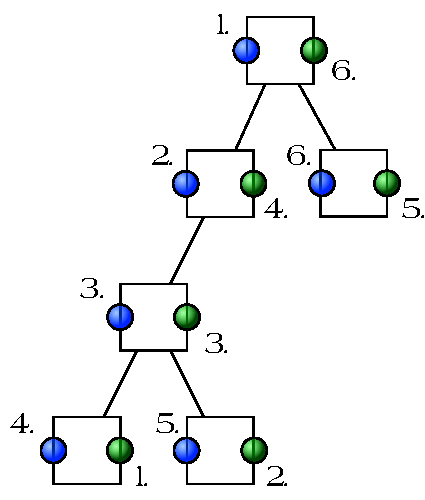
\includegraphics[width=0.4\linewidth]{traversal_mode.pdf}
 \caption{An illustration of the pre- and post-order traversal strategies: the blue points show the order in which the tree gets transformed in pre-order traversal, and the green ones illustrate the post-order traversal. Instead of pre- and post-order, we can also think of the transformations being applied top-down or bottom-up, hence the $\downarrow$ and $\uparrow$ aliases.}
 \label{figure:traversal_mode}
\end{figure}

As a first example, let us write and use a transformation that replaces all trees in the AST which do not have a range position with the \src{EmptyTree}.

\begin{lstlisting}
val tree: Tree = %\ldots%

val emptyTree = transformation[Tree, Tree] {
  case t if t.pos.isRange => t
  case _ => EmptyTree
}

preorder(allChildren(emptyTree)) apply tree
\end{lstlisting}

Preorder traversal already applies the transformation to all children, so we can simplify this to:

\begin{lstlisting}
preorder(emptyTree) apply tree
\end{lstlisting}

Of course, this is not the only way to achieve this, here is a variation that separates the testing for the range position into a predicate and uses a simple transformation to replace the tree. If the tree has a range position, it is not transformed (remember that the \src{id} transformation simply returns its argument unchanged). In case the predicate fails, the tree is replaced.

\begin{lstlisting}
val hasRangePosition = predicate((t: Tree) => t.pos.isRange)

val emptyTree = transformation[Tree, Tree] {
  case _ => EmptyTree
}

preorder(hasRangePosition &> id[Tree] |> emptyTree) apply tree
\end{lstlisting}

Using the \src{not} combinator, we can swap the two actions:

\begin{lstlisting}
preorder(not(hasRangePosition) &> emptyTree |> id[Tree]) apply tree
\end{lstlisting}

To get rid of the \src{id} transformation, we can use a different traversal strategy for the children:

\begin{lstlisting}
preorder(matchingChildren(not(hasRangePosition) &> emptyTree)) apply tree
\end{lstlisting}

More examples can be found in Section \vref{subsection:tree-transformations}.

\subsection{Creating Trees}

Most refactorings do not just reuse existing trees but also have to create new ones. The Scala compiler already contains several facilities to create new trees: the trait \src{scala.tools.nsc.ast.Trees} contains many methods that create AST trees and there's even a DSL in \src{scala.tools.nsc.ast.TreeDSL} whose ``goal is that the code generating code should look a lot like the code it generates'' \cite{TreeDSL}.

An example from \src{Trees} shows how many methods there are to create method definitions (this code has obviously been written before Scala had default arguments):

\begin{lstlisting}
def DefDef(sym: Symbol, mods: Modifiers, vparamss: List[List[ValDef]], rhs: Tree): DefDef

def DefDef(sym: Symbol, vparamss: List[List[ValDef]], rhs: Tree): DefDef
  
def DefDef(sym: Symbol, mods: Modifiers, rhs: Tree): DefDef

def DefDef(sym: Symbol, rhs: Tree): DefDef

def DefDef(sym: Symbol, rhs: List[List[Symbol]] => Tree): DefDef
\end{lstlisting}

Using the TreeDSL allows one to write very concise code. The following listing creates the AST for the code that checks whether \src{tree} is null.

\begin{lstlisting}
IF (tree MEMBER_== NULL) THEN %\ldots% ELSE %\ldots%
\end{lstlisting}

Unfortunately, all these tree construction helpers are problematic for us: they can change the position of the trees, which we have to avoid when we want to retain the source code layout. For this reason, the refactorings do not make use of these facilities but simply create the trees from scratch. There are some helper methods in \src{transformation.TreeFactory} which take care of constructing trees that are needed by the currently implemented refactorings:

\begin{lstlisting}
def mkRenamedSymTree(t: SymTree, name: String): SymTree

def mkReturn(s: List[Symbol]): Tree

def mkValDef(name: String, rhs: Tree): ValDef

def mkCallDefDef(name: String, arguments: List[List[Symbol]], 
  returns: List[Symbol]): Tree

def mkDefDef(mods: Modifiers, name: String, 
  parameters: List[List[Symbol]], body: List[Tree]): DefDef

def mkBlock(trees: List[Tree]): Block
\end{lstlisting}

Now that we have seen how trees can be transformed and how new trees can be generated, we are ready for a larger example.

\subsection{Tree Transformations}\label{subsection:tree-transformations}

For the usage in the refactoring, the \src{TreeTransformations} trait implements the traversal for Scala's AST and provides some definitions that make writing transformations more concise:

\begin{lstlisting}
def transform(f: PartialFunction[Tree, Tree]) = transformation(f)
  
def filter(f: %$\Rightarrow$% PartialFunction[Tree, Boolean]) = predicate(f)
\end{lstlisting}

Let us now take a look at a larger example: Extract Method. At the beginning of this section, we looked at the different transformations that occur during the refactoring: Insert a new method with the extracted statements and replace them with a call to this new method. This can be achieved with the following transformations:

\begin{lstlisting}
val replaceBlockOfStatements = transform {
  case block @ BlockExtractor(stats) => {
    mkBlock(stats.replaceSequence(selectedTrees, callExtractedMethod))
  }
}

val replaceSingleExpression = transform {
    case t if t == selectedTree => callExtractedMethod
}

val replace = topdown {
  matchingChildren {
    if(extractSingleTree)
      replaceSingleExpression
    else
      replaceBlockOfStatements
  }
}

val insertExtractedMethod = transform {
  case tpl @ Template(_, _, body) => 
    tpl copy (body = body ::: extractedMethod :: Nil) setPos tpl.pos
}
\end{lstlisting}

A remark on the call to \src{setPos tpl.pos} in \src{insertExtractedMethod}: Because the structure of a tree is immutable, we cannot change a tree in-place, even though we often want to do this. The source regeneration uses the position information of the trees to determine whether a tree's existing source code can be reused. So if we want a tree to appear modified in-place, we simply assign it the position of the original tree. Note that this does only work if the two trees are of the same type.

Next we need two filters that find the enclosing class' template and the method we extract from:

\begin{lstlisting}
val findTemplate = filter {
  case Template(_, _, body) => body exists (_ == selectedMethod)
}

val findMethod = filter {
  case d: DefDef => d == selectedMethod
}
\end{lstlisting}

Now we can combine these to assemble a new transformation that performs the following steps:

\begin{enumerate}
 \item Traverse the tree until the selected template is found, the one that contains \src{selectedMethod}.
 \item Once we found the template, start the following two transformations:
  \begin{enumerate}
        \item Find the method we extract from and apply the \src{replace} transformation on it.
        \item Insert the new method in the class template.
       \end{enumerate}
\end{enumerate}

%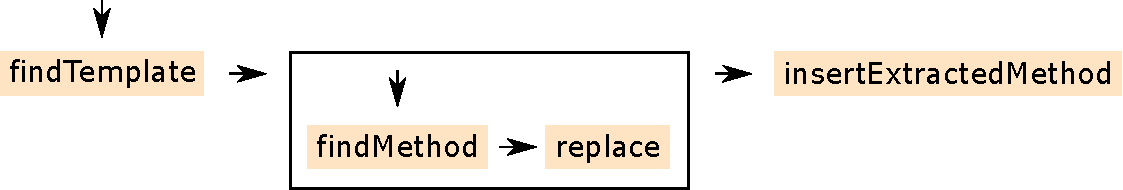
\includegraphics[width=\linewidth]{extract_method_transformation.pdf}

All these steps can be expressed with a simple transformation:

\begin{lstlisting}
val extractMethod = topdown {
  matchingChildren {
    findTemplate &> 
    topdown {
      matchingChildren {
	findMethod &> replace
      }
    } &> 
    insertExtractedMethod
  }
}
\end{lstlisting}

\section{Source Generation}\label{section:source-generation}

Once our abstract syntax tree has been refactored, we need to convert it back into its textual source code representation. This process comprises two main steps: the \textit{detection of modifications} to minimize the amount of code that is regenerated and the actual \textit{source generation}.

The first step is necessary because we -- in contrast to many other refactoring implementations -- do not keep track of modifications to the AST while they are happening but reconstruct this information afterwards. This allows us to keep the transformations simpler but consequently makes the code generation more complex. This tradeoff is worthwile because we intend the library to be reused and the transformations to be implemented by third parties.

The AST after the refactoring may contain several kinds of modifications. Trees can be moved around, deleted and new trees can be introduced. From the transformations we know that trees that are moved around keep their original position information, and newly created trees have a \src{NoPosition} attribute per default. This allows us to detect changes and can later be used during source generation to preserve the layout of already existing trees. 

\subsection{Modification Detection}

The primary goal of a fine-grained modification detection is to reduce the amount of trees that are regenerated. The source generation is invoked with a list of trees from various files that all can have an arbitrary number of changed children:

\begin{lstlisting}
def createChanges(ts: List[Tree]): Iterable[Change]
\end{lstlisting}

Modification detection performs the following three steps on the input trees:

\begin{enumerate}
 \item Group all changed trees by their file.
 \item Find the top-level changed trees for each file.
 \item Detect the change-set per top-level tree.
\end{enumerate}

Top-level trees are trees that are ancestors of other changed trees. For example, the following graph shows an AST with some changed trees in green and blue:

\begin{center}
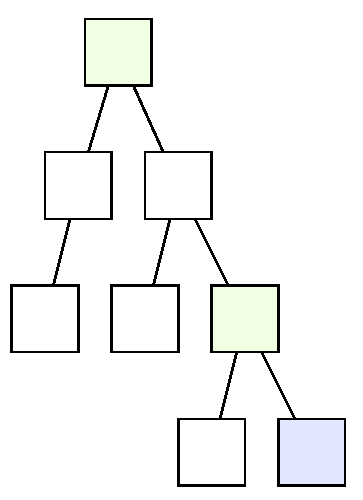
\includegraphics[width=0.2\linewidth]{ast_with_changes.pdf}
\end{center}

The \src{createChanges} method is invoked with the two green trees, but the blue tree has also been modified by a transformation.

Now if we were to generate two changes from the two green trees, we would get a problem when applying the changes because they overlap each other. The two changes would either overwrite each other or, in the case of Eclipse's Language Toolkit, yield an error. Therefore the second step of the modification detection is to find those trees that contain other changed trees. In the AST above, this would be the root node.

The third step then traverses these top-level trees and finds all changes as well as the trees that lie between changed trees, here marked in blue:

\begin{center}
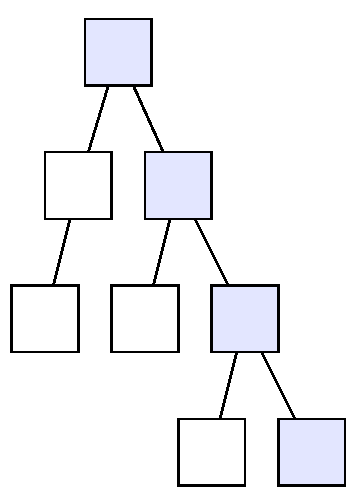
\includegraphics[width=0.2\linewidth]{ast_with_changeset.pdf}
\end{center}

This set of trees is the minimal number of trees that need to be regenerated. Trees that are not contained in the set can be kept as they are to improve the performance. \figref{figure:ast_with_changes_large} shows a larger example of the process.

\begin{figure}
 \centering
 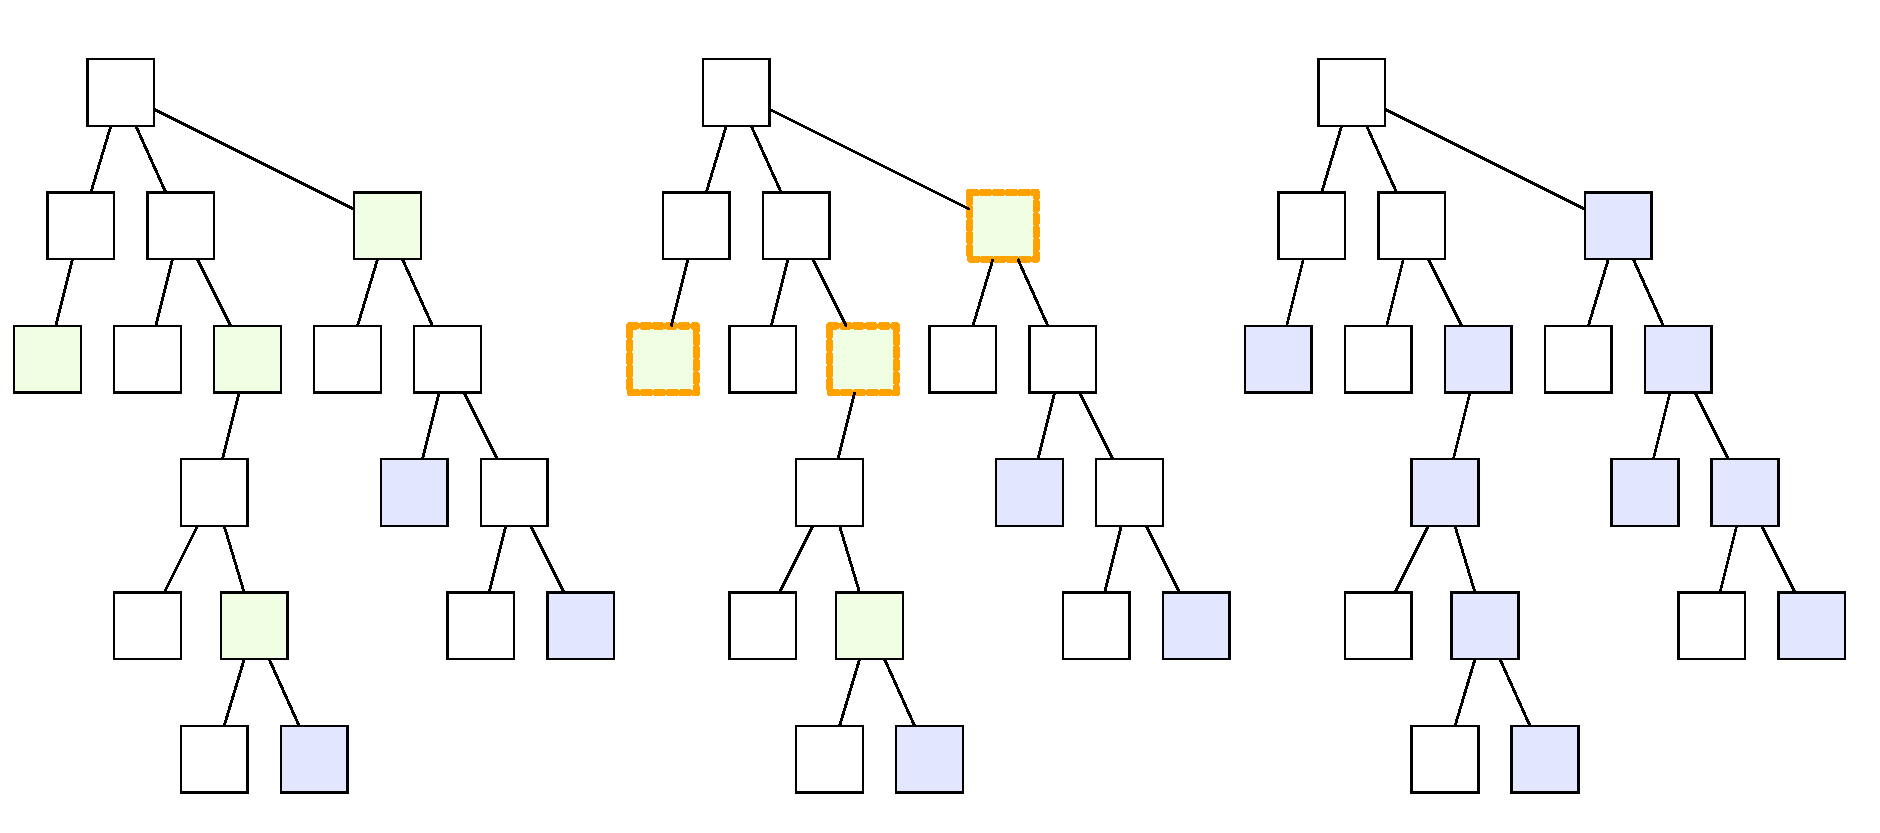
\includegraphics[width=\linewidth]{./ast_with_changes_large.pdf}
 \caption{An example of how the change set is built: the left AST shows in green the list of all trees that should be regenerated, but the blue trees have changed as well. In the middle graph, we see the trees that were identified as top-level trees. The rightmost AST shows all trees that need to be regenerated.}
 \label{figure:ast_with_changes_large}
\end{figure}

Once we have identified all top-level tree changes, we start generating source code for them. 

\subsection{Code Generation}

The AST does -- by its very nature -- not contain all the information that is necessary to fully reconstruct its original textual representation. Also, syntactic sugar of the programming language is typically not represented in the AST; only the desugared representation is preserved. An example for this are Scala's \src{for} comprehensions. Because they are equivalent with function calls to \src{map, filter, flatMap,} and \src{foreach}, there is no need to create additional tree classes for them. This means that the two statements in the following listing have the same representation in the AST.

\begin{lstlisting}
val v1 = List(1,2,3) map (i => i * 2)
val v2 = for(i <- List(1,2,3)) yield i * 2
\end{lstlisting}

Other things that are not mentioned explicitly in the AST are parenthesis, commas and many other tokens. In the context of source generation, we will call them layout elements, or just \textit{layout}. 

If we were only interested in a semantically equivalent program, we could simply pretty print the AST to generate the source code. A purely AST based pretty printer would unknowingly convert the user's \src{for} comprehensions from above into the \src{map} form. No user of a refactoring tool would accept this, and this is also not the only problem: because comments in the source code are generally considered whitespace by parsers, they are not represented in the AST and get lost during pretty printing (see \cite{RetainingComments} for a detailed treatment of this particular problem). It is clear that we need a more refined technique.

The original source code is always available to the refactoring tool, and with the position information on the trees, we have a means to look up the original source code for a tree.

Other refactoring tools (e.g. the C++ Development Tooling for Eclipse \cite{CdtOopsla} or the Ruby Development Tools \cite{RubyOopsla}) have used various approaches to solve this problem (XX ref to old doku). For some cases -- for example in a rename refactoring -- it might even be acceptable to pretty print the code as long as only very small regions of the program change. This approach can be problematic -- for example with the Extract Method refactoring, where arbitrary large parts of the program are moved around. A tool can handle this situation by cut-and-pasting the body of the extracted method. This is not feasible for us because we need a generic way to handle all kinds of unforseeable changes to the source code.

\subsubsection{Preserving Layout}

Our approach is based on using two different kinds of source printers: one that pretty prints code  and another one that reuses the existing code where possible. The \textit{pretty printer} simply prints the code with a default layout and is used for trees that were introduced during the transformation. The \textit{reusing printer} takes the existing layout with the help of the trees's position information and also makes sure all needed layout elements are present. How this is done will be explained in more detail later.

The source generation algorithm then alternates between these two printers during the code generation process.

Now we just need to know how we can reuse the existing layout. What we need is a way to decide how all these layout elements can be associated to their enclosing trees. If we take a look at the following listing, we can see several occurences of whitespace and other layout, like the three comments and the braces.

\begin{lstlisting}
package p //TODO
// myclass
class MyClass(a: Int /* the int */) {
}
\end{lstlisting}

Because no rules of the programming language dictate how the layout is associated with the other parts of the program, we have to guess how to divide it and associate it with its surrounding trees. Often this can be done by taking the types of the adjacent trees into consideration and then divide the layout according to some rules and regular expressions. 

For example, one rule says that the layout between two enclosing value definitions is split by a comma, or by newline if there is no comma present. So when the values are part of an argument list, they will get comma-separated, and if they are definitions, the layout will be split at the end of the line, so that the first value will get all layout that follows on its line. Comments can be handled with the same rules as well: a comment on a preceding and otherwise empty line is associated with the following tree.

Let us take a look at a concrete example. \figref{figure:ast_with_layout} shows the AST of the previous listing and how the layout elements have been associated with the left and right sides of a tree. Note that the \src{class} and \src{package} keywords are also considered layout, this is because they are not represented in the AST with their own tree and position information.

\begin{figure}
 \centering
 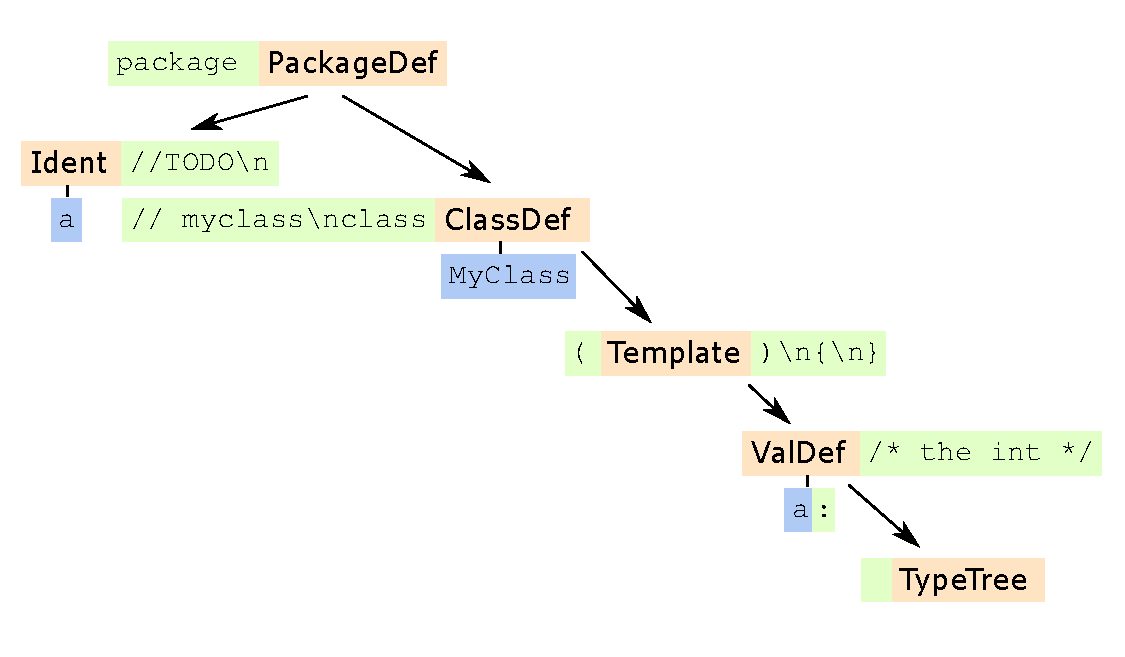
\includegraphics[width=0.8\linewidth]{ast_with_layout.pdf}
 \caption{An example of how layout can be associated with trees: the apricot colored boxes represent the trees and the green ones their associated layout. The blue parts are not real AST nodes but names; they are treated like trees in the source generation.}
 \label{figure:ast_with_layout}
\end{figure}

Once we have identified the layout that belongs to a tree, we can use it during the source generation. For example, it should be clear now that when we would delete the \src{ValDef} parameter in the above AST, then the comment would be removed along with it.

Another issue that concerns both the pretty and the reusing printer is the indentation of the code. When a new statement in a block of other statements is inserted, we want it to have the same indentation as its siblings. For this, the printers also keep track of the currently desired indentation as specified by the parent tree. 

Whether we can reuse existing code or have to invoke the pretty printed needs to be decided for each tree in the AST. This gives us the following definition of the various source printers:

\begin{lstlisting}
trait AbstractPrinter {
  def print(t: Tree, ind: Indentation): Fragment
}

trait PrettyPrinter extends AbstractPrinter {
  def print %\ldots%
}

trait ReusingPrinter extends AbstractPrinter {
  def print %\ldots%
}

trait SourceGenerator extends PrettyPrinter with ReusingPrinter {
  override def print(t: Tree, i: Indentation): Fragment = {
    if(t.hasExistingCode)
      super[ReusingPrinter].print(t, i)
    else if(t.hasNoCode)
      super[PrettyPrinter].print(t, i)
    else
      EmptyFragment
  }
%\ldots%
\end{lstlisting}

\subsubsection{Fragments and Layout}

The result of a printing operation is not a plain string but an instance of \src{Fragment}. A fragment contains a leading, center, and trailing layout. A layout is simply a wrapper around a string or a part of the source file with some additional helper methods. For example, in \figref{figure:ast_with_layout}, all the apricot and blue colored boxes are fragments and the green ones are instances of \src{Layout}.

The fragments and layouts are created in the printers, where they pattern match on the tree and recursively print the children of a tree. This is an excerpt from the pretty printer:

\begin{lstlisting}
def print(t: Tree, ind: Indentation) = t match {
  case PackageDef(pid, stats) =>
    Layout("package ") ++ 
      printTree(pid, after = newline) ++ 
      printTrees(stats, separator = newline)
%\ldots%
\end{lstlisting}

The \src{++} operation on the layout and the fragments simply concatenate their operands, again yielding a fragment. So far, we could also have just used plain Strings and concatenate them with \src{+}, except that using strings weakens the typesystem because every object can be concatenated to a String using the implicit \src{toString} method.

\subsubsection{Reusing Layout}

The printers also have to take care that all the necessary layout is printed when needed. This can become difficult when layout is reused. Imagine the following scenario: We create a new \src{Block} (a \src{Block} tree wraps a list of other statements) and insert several statements into it. The pretty printer separates each statement in a block with a newline, so the code to pretty print a block could look like this:

\begin{lstlisting}
case Block(stats) =>
  Layout("{"+newline) ++ 
    printTree(stats, separator = newline) ++ 
    Layout(newline+"}")
\end{lstlisting}

This works fine as long as the statements are not reused trees that might already have a leading or trailing newline in their associated layout. If this is the case, we could get too many blank lines between our statements. 

To solve this, the pretty printer could print the block's children one by one and then check if the newline is already present or needs to be inserted. This is tedious to do in every place where a layout element is inserted, so we need a more generic way to handle such cases, and this is where the \src{Requisites} come into play. Instead of specifying the layout directly, the printers simply declare that there needs to be a newline present in the surrounding layout:

\begin{lstlisting}
case Block(stats) =>
  Requisite("{"+newline) ++ 
    printTree(stats, separator = Requisite(newline)) ++ 
    Requisite(newline+"}")
\end{lstlisting}

Now during the concatenation of fragments and layout objects with \src{++}, it is checked whether a certain requisite is already satisfied. The layout is only generated when it is nedeed.

This leads us to the following three interfaces (the \src{++} operators and some other methods have been omitted) that are used to represent the source code in the printers:

\begin{lstlisting}
trait Layout {
  def asText: String
}

trait Requisite {  
  def isRequired(l: Layout, r: Layout): Boolean
  def apply(l: Layout, r: Layout): Layout
}

trait Fragment {
  def leading:  Layout
  def center:   Layout
  def trailing: Layout
  
  def pre: Requisite
  def post: Requisite
  
  def asText: String
}
\end{lstlisting}

Using implicit conversions (XX anhang), short aliases for the print methods and Scala's named and defaul arguments, this allows us to write the code for the two printers in a very concise way. Pattern matching gives us the ability to easily handle special cases and variations, as can be seen from the \src{Bind} matches below:

\begin{lstlisting}
trait PrettyPrinter  {
  
  def print %\ldots%  

    case Alternative(trees) =>
      p(trees, separator = " | ")
      
    case Star(elem) =>
      p(elem) ++ Layout("*")
      
    case Bind(name, body: Typed) =>
      Layout(name.toString) ++ p(body, before = ": ")

    case Bind(name, body: Bind) =>
      Layout(name.toString) ++ p(body, before = " @ \\(", after = "\\)")
      
    case Bind(name, body) =>
      Layout(name.toString) ++ p(body, before = " @ ")
    %\ldots%
}
\end{lstlisting}

\subsection{Using the Source Generator}

For users of the code generation, there are several methods to transform a tree back into source code. The \src{createChanges} method of the \src{SourceGenerator} trait creates the change objects from a list of trees by first narrowing down the changed trees and then generating the code for them:

\begin{lstlisting}
def createChanges(ts: List[Tree]): List[Change]
\end{lstlisting}

The result is a list of change objects that describe which parts in a file are to be replaced:

\begin{lstlisting}
case class Change(file: AbstractFile, from: Int, to: Int, text: String)
\end{lstlisting}

This is the preferred method for IDEs that operate with change objects. The \src{Change} object contains a useful function that applies a list of changes to a source code string:

\begin{lstlisting}
def applyChanges(ch: List[Change], source: String): String
\end{lstlisting}

Alternatively, if one just wants to generate the source code from a tree, the \src{createFragment} method can also be invoked directly. 

\begin{lstlisting}
def createFragment(t: Tree): Fragment
\end{lstlisting}
